\section{Approach}
\label{sec:approach}

Our approach accepts a set of projects as data sources and mines
API mapping between two different languages $L_1$ and $L_2$.
As mined API mapping describes mapping relations of APIs between
the two languages, this mapping is useful for language migration between the two languages.
For each project used as a data source, our approach requires
atleast two versions of the project (one version in $L_1$ and
the other version in $L_2$). Figure~\ref{fig:approach} shows
the overview of our approach.

First, our approach aligns client code in languages $L_1$ and $L_2$
so that the aligned source files implement similar functionalities
(Section~\ref{sec:approach:acc}). Second, our approach mines
mapping relations of API classes (Section~\ref{sec:approach:mappingtypes}).
Finally, our approach mines mapping relations of API
methods (Section~\ref{sec:approach:mappingtypes}) defined by the mapped
API classes.

\begin{figure}[t]
\centering
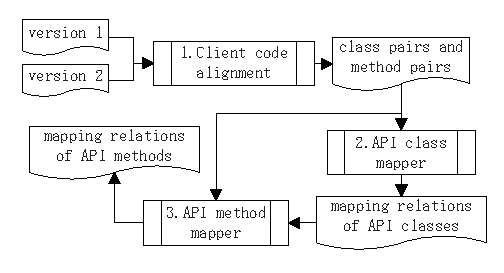
\includegraphics[scale=1,clip]{figure/approach.eps}\vspace*{-3ex}
 \caption{Overview of our approach}\vspace*{-3.5ex}
 \label{fig:approach}
\end{figure}

%-------------------------------------------------------------------
\subsection{Aligning Client Code}
\label{sec:approach:acc}

Initially, our approach accepts two versions of a project (one version in
$L_1$ and the other version in $L_2$) and aligns classes and methods
of the two versions. Aligned classes or methods
between the two versions implement a similar functionality. As they
implement a similar functionality, APIs used by these classes or methods can be
replaceable.

To align classes and methods of the two versions, our approach uses
name similarities between entities (such as class names or method names)
defined by the two versions of the project. In our approach, we have two
different kinds of entity names: entity names defined by the two versions
of the project and entity names of third-party libraries used by the two versions of the project.
The first kind often comes from the same programmer or the same team, or
programmers may refer to existing versions for naming entities such
as classes, methods, and variables. Therefore, name similarity is often
reliable to distinguish functionalities of the first kind compared to the second
kind. Our approach uses Simmetrics\footnote{\url{http://sourceforge.net/projects/simmetrics/}}
to calculate name similarities.

Algorithm 1 shows how our approach aligns client code classes. The
first step is to find candidate class pairs by names. For two sets
of classes ($C$ and $C'$), the algorithm returns candidate class
pairs ($M$) with a similarity greater than a given threshold,
referred to as \emph{SIM\_THRESHOLD}. As some projects may have many
classes with the same name, $M$ may contain more than one matching
pair for a class in a version. To align those classes, our algorithm
uses package names of these classes to refine $M$ and returns only
one matching pair with the maximum similarity\footnote{For C\#, we
refer to namespace names for package names.}.

In each aligned class pair, our approach further aligns methods
within the class pair. The algorithm for methods is similar to the
algorithm for classes but relies on other criteria such as the number of parameters
and names of parameters to refine candidate method pairs. These candidates
may contain more than one method pair due to overloading.
For the example shown in Section~\ref{sec:example}, our approach
correctly aligns the class \CodeIn{IndexFiles} and the method
\CodeIn{main} in Java to the class \CodeIn{IndexFiles}
and the method \CodeIn{Main} in C\# as their names are quite
similar.
%-----------------------------------------------------------------
\subsection{Mapping API classes}
\label{sec:approach:mappingtypes}

In this step, our approach mines mapping relations of
API classes. As defined in Section~\ref{sec:mapping}, mapping relations of API classes are used
to translate variables. Consequently, our approach mines mapping
relations of API classes based on how aligned client code declares
variables such as fields of aligned classes, parameters of aligned methods
and local variables of aligned methods. In
particular, for each aligned class pair $\Pair{c_1} {c_2}$, our
approach analyzes each field pair $\Pair{f_1}{f_2}$ and considers
$\Pair{f_1.type} {f_2.type}$ as one mined mapping relation of API
classes when the similarity between $f_1.name$ and $f_2.name$ is
greater than \emph{SIM\_THRESHOLD}. Similarly, for each aligned method pair
$\Pair{m_1} {m_2}$, our approach analyzes each local variable pair
$\Pair{var_1} {var_2}$ and considers $\langle var_1.type,$ $
var_2.type\rangle$ as one mined mapping relation of API classes when
the similarity between $var_1.name$ and $var_2.name$ is greater than
a threshold. Also, our approach analyzes each parameter pair
$\langle para_1, $ $para_2\rangle$ of $m_1$ and $m_2$, and our
approach considers $\langle para_1.type,$ $para_2.type\rangle$ as
one mined mapping relation of API classes when the similarity
between $para_1.name$ and $para_2.name$ is greater than \emph{SIM\_THRESHOLD}.

For the example shown in Section~\ref{sec:example}, our approach
mines the mapping relation between \CodeIn{java.io.File} and
\CodeIn{System.IO.FileInfo} based on the matched fields of Lines 4
and 9 (Figure~\ref{fig:clientcode}). The mapping relation of API classes helps translate the
variable declared in Line 1 (Figure~\ref{fig:totranslation})
to the variable declared in Line 16 (Figure~\ref{fig:translatedcode}).

%\begin{algorithm}[t]
%\begin{SmallOut}
%\dontprintsemicolon
%  \KwIn{$C$ is the classes of a language; $C'$ is the classes
%  of another language}
%  \KwOut{$P$ is aligned pairs of classes}
%  \Begin{
%     $M \leftarrow findCandidateClassPairs(C, C')$\;
%     \While{$M.size > 0 $}{
%        \If{$M.size > 1$}{
%            $M \leftarrow refineByPackageNames(M)$\;
%         }
%         \If{$M.size == 1$}{
%                $P.add(M)$\;
%                $C.remove(M[0].c)$\;
%                $C'.remove(M[0].c')$\;
%         }
%         $M \leftarrow findCandidateClassPairs(C, C')$\;
%     }
% }
%\end{SmallOut}
%\label{alg:alignclasses} \caption{Align Classes Algorithm}
%\end{algorithm}

\begin{figure}[t]
\centering
\includegraphics[scale=1,clip]{figure/algorithm1.eps}
\vspace*{-6ex}
\end{figure}

%-----------------------------------------------------------
\subsection{Mapping API methods}
\label{sec:approach:mappingtypes}

In this step, our approach mines mapping relations of API methods.
This step has two major sub-steps. First, our approach builds a graph, referred
as API transformation graph, for each client code
method. Second, our approach compares the two graphs of each paired
client code methods for mining mapping relations of API methods.

\begin{figure*}[t]
\centering
\includegraphics[scale=1.1,clip]{figure/graph.eps}\vspace*{-3ex}
 \caption
{\label{fig:graph}Built ATGs and the main steps of comparing
ATGs}\vspace*{-3.5ex}
\end{figure*}


\subsubsection{API transformation graph}
We propose API transformation graphs (ATG) to help deal with the two
challenges of mining API mapping listed in
Section~\ref{sec:introduction}. An API transformation graph of a
client code method $m$ is a directed graph
$G\Triple{N_{data}}{N_{m}}{E}$. $N_{data}$ is a set of the fields
$F$ of $m$'s declaring class, local variables $V$ of $m$, parameters
$P_1$ of $m$, parameters $P_2$ of methods called by $m$, and return
values $R$ of all methods. $N_{m}$ is a set of methods called by
$m$. $E$ is a set of directed edges. An edge $d_1\rightarrow d_2$
from a datum $d_1 \in N_{data}$ to a datum $d_2 \in N_{data}$
denotes the data dependency from $d_1$ to $d_2$. An edge $d_1
\rightarrow m_1$ from a datum $d_1 \in N_{data}$  to a method $ m_1
\in N_{m}$ denotes $d_1$ is a parameter or a related variable of
$m_1$. An edge $m_1 \rightarrow d_1$ from a method $m_1 \in N_{m}$
to a datum $d_1 \in N_{data}$ denotes $d_1$ is the return value of
$m_1$.

%We propose ATG for two main purposes. The first purpose is to mine mapping
%relations among parameters of mapped API methods. Mining mapping relations
%among parameters of mapped API methods is challenging as often mapped API methods
%can have different number of parameters or different positions among
%parameters. For example, consider the following two mapped API methods:
%
%\begin{CodeOut}
%$m_1$ in Java: BigDecimal java.math.BigDecimal.multiply (BigDecimal $p_1^1$)\\
%\hspace*{0.11in}$m_2$ in C\#: Decimal System.Decimal.Multiply (Decimal $p_1^2$, Decimal $p_2^2$)
%\end{CodeOut}
%
%Method $m_1$ of Java has a receiver variable, say $v_1^1$, of type \CodeIn{BigDecimal}
%and has one parameter $p_1^1$. The mapped method $m_2$ in C\# has
%two parameters $p_1^2$ and $p_2^2$. Using ATGs, our approach
%identifies that $v_1^1$ is mapped to $p_1^2$ and $p_1^1$ is mapped
%to $p_2^2$. As ATG captures parameters of API methods,
%our approach is able to deal with the challenges of mapping parameters.
%
%The second purpose of ATG is to mine mapping relations of merged API methods. As ATG
%describes data dependencies among inputs and outputs, our approach
%is able to mine mapping relations for merged API methods as shown in
%Figure~\ref{fig:example}. We next describe how our approach builds ATGs and
%uses ATGs for mining mapping relations of API methods.

\subsubsection{Building API transformation graphs }

Our approach builds an ATG for each method $m$. ATG includes information such as
inputs and outputs for each client code method. In particular, for
each method $m$, our approach first builds subgraph for its variables,
API methods, and field accesses according to the following rules:

%First, programming languages typically provide a huge set of APIs,
%and it is difficult to build mapping relations for all APIs
%manually. Second, some API methods have multiple parameters, and
%some parameters cannot be mapped directly one by one in orders. For
%example, \CodeIn{org.w3c.dom.Element.getAttributeNS()} and
%\CodeIn{System.Xml.XmlElement.GetAttribute()} both have two
%parameters, but the two parameters are inverse by their meanings.
%Third, one API method in one language may be mapped to more than one
%API method in other languages. For example, \CodeIn{java.util.
%LinkedList.removeLast()} returns the last value, and \CodeIn{System.
%Collections.Generic.LinkedList.RemoveLast()} does not return any
%values. To get that value, C\# programmers need to call more APIs,
%and thus one API method of Java is mapped to serval API methods of
%C\#.



%
%One challenge to mine mapping relations of two API methods lies in
%how to map their inputs correctly. Here, our approach both the
%receiver and the parameters of a method as the inputs of a
%method. Inputs of two API methods may be matched but are not in the
%same order. For example, as shown in Section~\ref{sec:example},
%\CodeIn{java.io. File.exist()} has a receiver whereas
%\CodeIn{System.IO.File.Exist()} has no receiver but a
%parameter. In addition, parameter orders may be quite different. For
%example, the parameter order of \CodeIn{org.w3c.
%dom.Element.getAttributeNS()} is inverse with the parameter order of
%\CodeIn{System.Xml.XmlElement.GetAttribute()}. To deal with the
%preceding problem,


\begin{enumerate}\vspace*{-2ex}
\item $\forall$ $f \in F \cup V \cup P_1$, our approach adds a node to the built ATG.
The reason for considering these variables such as fields in
declaring class or local variables in method $m$ used in client code
is that these variables are useful to analyze data dependencies
among API methods.\vspace*{-2ex}
%\begin{center}
%\includegraphics[scale=0.7,clip]{figure/rule1.eps}
%\end{center}
\item $\forall$ API methods of the form ``$T_0\ T.AM (T_1 p_1, \ldots, T_n p_n)$''
called by method $m$, our approach adds receiver (of type $T$) and
parameter nodes to the built ATG as shown below. Our approach does
not add receiver node for static API methods. \vspace*{-3ex}
\begin{center}
\includegraphics[scale=0.7,clip]{figure/rule2.eps}%\vspace*{-1.5ex}
\end{center}\vspace*{-3ex}
\item $\forall$ $f\in F \cup V$, if $f$ is a non-primitive variable
of type $T_1$ and a field $x$ of $T_1$ is accessed as $f.x$, our
approach adds nodes to the built ATG as shown below. As Java often
uses getters and setters whereas C\# often use field accesses, our
approach treats field accesses as a special type of method
calls.\vspace*{-2ex}
\begin{center}
\includegraphics[scale=0.7,clip]{figure/rule3.eps}%\vspace*{-1.5ex}
\end{center}\vspace*{-3ex}
\end{enumerate}

Our approach adds additional edges to the built ATG (and sub-graphs
inside ATG) representing data dependencies among built sub-graphs.
We use the following rules for adding additional edges to the built
ATG. \Comment{In particular, our approach analyzes source files of a
client code method statement by statement and adds edges according
to the rules as follows:} \vspace*{-1.5ex}
\begin{enumerate}
\item $\forall$ statements of the form $x = y$, where $x \in F \cup V \wedge y \in F \cup V$,
our approach adds an edge from $y$ to $x$. This edge represents that
$x$ is data dependent on $y$.\vspace*{-1.5ex}
\begin{center}
\includegraphics[scale=0.7,clip]{figure/rule4.eps}%\vspace*{-1.5ex}
\end{center}\vspace*{-1.5ex}
\item $\forall$ statements of the form $x = AM()$, where $x \in F \cup V$, our approach
adds an edge from $AM$ to $x$ if the return value of $AM$ is
assigned to $x$. This edge represents that $x$ is data dependent on
the return value of $AM$. \vspace*{-1.5ex}
\begin{center}
\includegraphics[scale=0.7,clip]{figure/rule5.eps}%\vspace*{-1.5ex}
\end{center}\vspace*{-1.5ex}
\item $\forall$ API methods $AM(x)$ called by method $m$, our approach
adds an edge from $x$ to the parameter node of $AM$. This edge
represents that the parameter of $AM$ is data dependent on
$x$.\vspace*{-1.5ex}
\begin{center}
\includegraphics[scale=0.7,clip]{figure/rule6.eps}%\vspace*{-1.5ex}
\end{center}\vspace*{-1.5ex}
\item $\forall$ statements of the form $m_2(m_1(x))$, our approach
adds an edge from the return value node of $m_1$ to the parameter
node of $m_2$ parameter node. This edge represents that the
parameter of $m_2$ is data dependent on the return value of
$m_1$.\vspace*{-1.5ex}
\begin{center}
\includegraphics[scale=0.7,clip]{figure/rule7.eps}%\vspace*{-1.5ex}
\end{center}\vspace*{-1.5ex}
\item $\forall$ statements of the form $x.m()$, our approach adds
an edge from $x$ to $m$ as $x$ is the receiver object of $m$. This
edge represents that the receiver object of $m$ is data dependent on
$x$.\vspace*{-1.5ex}
\begin{center}
\includegraphics[scale=0.7,clip]{figure/rule8.eps}%\vspace*{-1.5ex}
\end{center}\vspace*{-1.5ex}
\item $\forall$ statements of the form $ x = y\ op\ z\ op\ \ldots, op \in \{+,-,*,/\}$,
our approach adds edges from $y$, $z$, and others to $x$, as these
variables are connected by binary operations and the return value is
assigned to $x$. The edge denotes the data dependency from $y$, $z$,
and other variables to $x$. For simplicity, our approach ignores
\emph{op} info. We discuss the issue in
Section~\ref{sec:discuss}.\vspace*{-1.5ex}
\begin{center}
\includegraphics[scale=0.7,clip]{figure/rule9.eps}%\vspace*{-1.5ex}
\end{center}\vspace*{-2ex}
\end{enumerate}

For each method $m$ in the client code, our approach applies preceding
rules for each statement from the beginning to the end of $m$.
Within each statement, our approach applies these rules based on
their nesting depth in the abstract syntax tree. For example,
for the statements of the form $m_2(m_1(x))$, our approach first applies
these rules on $m_1$ and then on $m_2$.

Figures~\ref{fig:graph}a and ~\ref{fig:graph}b show partial ATGs for
C\# (\CodeIn{IndexFiles.cs}) and Java (\CodeIn{IndexFiles.java})
code examples shown in Figure~\ref{fig:clientcode}, respectively.
Figure~\ref{fig:graph} also shows corresponding line numbers of each
sub-graph. Our approach applies Rules 2 and 6 for Lines 4 and 9 (Figure~\ref{fig:clientcode})
to build corresponding sub-graphs in the ATG. For
Lines 6 and 7 (Figure~\ref{fig:clientcode}), our approach applies Rules 2 and 8 to build
corresponding sub-graphs in the ATG. For Lines 12 and 15 (Figure~\ref{fig:clientcode}),
our approach applies Rule 2, 3, and 6 to build corresponding sub-graphs.

%\begin{algorithm}[t]
%\begin{SmallOut}
%\label{alg:mapATG} \dontprintsemicolon
%  \KwIn{$G$ is the ATG of a method ($m$); $G'$ is the ATG of $m$'s mapped method.}
%  \KwOut{$S$ is a set of mapping relations for API methods}
%  \Begin{
%     $P \leftarrow findVarPairs(m, m')$\;
%     \For{Pair p in P}{
%        $SM \leftarrow G.nextMethods(p.sharp)$\;
%        $JM \leftarrow G.nextMethods(p.java)$\;
%        $\Delta S = mapping(SM, JM)$\;
%        \While{$\Delta S \neq \phi| \Delta SM \neq \phi| \Delta JM \neq \phi$}{
%            $S.addAll(\Delta S)$\;
%             \For{Method sm in SM}{
%                 \If{$sm.isMapped$}{
%                    $SM.replace(sm, sm.nextMethod())$\;
%                  }\Else{
%                    $SM.replace(sm, sm.mergeNextMethod())$\;
%                  }
%             }
%             \For{Method jm in JM}{
%                 \If{$jm.isMapped$}{
%                    $JM.replace(jm, jm.nextMethod())$\;
%                  }\Else{
%                    $JM.replace(jm, Jm.mergeNextMethod())$\;
%                  }
%             }
%             $\Delta S = mapping(SM, JM)$\;
%        }
%     }
% }
% \end{SmallOut}
%\caption{ATG Comparison Algorithm}
%\end{algorithm}

\begin{figure}[t]
\centering
\includegraphics[scale=1,clip]{figure/algorithm2.eps}
\vspace*{-6ex}
\end{figure}

%--------------------------------------------------------------------
\subsubsection{Comparing API transformation graphs}

The second sub-step compares each pair of built ATGs for mining mapping
relations of API methods. Our mapped API methods satisfy three
criteria: (1) Mapped API methods implement the same
functionality. (2) Mapping relation describes the relation
between parameters of mapped API methods. (3) Mapping relation
describes the relation between return values of
mapped API methods. The two mapped API methods in two
different languages satisfying the preceding three criteria
are replaceable in the client code. Therefore, these mapped API
methods assist for migrating client code from one language to another.

Algorithm 2 presents major steps of comparing ATGs for mining
mapping relations of API methods. Consider two methods $m$ and $m'$
of two different languages $L$ and $L'$, respectively, in the client
code. Consider that the associated ATGs of $m$ and $m'$ are compared
to mine mapping relations of API methods. First, our algorithm finds
matching variables $\in$ $F$, $V$, and $P_1$ in $m$ and $m'$. Our
algorithm maps two variables $v$ and $v'$ of methods $m$ and $m'$,
respectively, if the similarity measure on their names is greater
than \emph{SIM\_THRESHOLD}. For constants in $m$ and $m'$, our
algorithm maps those two constants, if they have exactly the same
value. Our algorithm uses these variable and constant mappings to
compute mappings between API methods that use these variables and
constants. Our algorithm uses the following criteria for mapping two
API methods $jm$ and $sm$.

\emph{Matching entities}: The first criterion is based on entities such as receiver variable
or parameters of $jm$ and $sm$ to map $jm$ and $sm$. We map $jm$ with $sm$, if
the receiver variable of API method $jm$ is mapped
to the receiver variable of $sm$, and there is a one-to-one mapping between parameters
of $jm$ and $sm$.

\emph{Matching functionalities}: The second criterion is based on functionalities of
$jm$ and $sm$. We consider that $jm$ and $sm$ implement the same functionality,
if the similarity measure between the name of $jm$ and the name of $sm$ is
greater than \emph{SIM\_THRESHOLD}.

\emph{Matching outputs:} The third criterion is based on the return values of $jm$ and $sm$.
Consider the return values of $jm$ and $sm$ as $r_1$ and $r_2$, respectively. We map $jm$
with $sm$, if the type of $r_1$ is mapped with the type of $r_2$ in mapping API classes
relationship.

Our algorithm first attempts to map first API method $jm$ in $m$
with the first API method $sm$ in $m'$. If our algorithm successfully maps $jm$ with
$sm$, our algorithm moves to the next available API methods in $m$
and $m'$ of the client code. If our algorithm does not able to map $jm$
with $sm$, our algorithm merges $sm$ and $jm$ with their next available API methods
in the corresponding ATGs, respectively, and attempts to map merged API methods.
For two merged API methods, our algorithm uses the
maximum similarity of method names between $jm$ and $sm$ as a
similarity measure for matching their functionalities.
With each iteration, $sm$ or $jm$ or the mapping relation (represented as $S$)
in the algorithm changes. Therefore, we repeat our algorithm
till $S$, $sm$, and $jm$ do not change anymore.

We next explain our algorithm using the illustrative example shown
in Figure~\ref{fig:graph}. The numbers shown in circles
represent the major steps in our algorithm for mining mapping
relations of API methods. We next explain each step in detail.

\emph{S1: mapping parameters, fields, local variables, and constants.}
Given two ATGs of each method pair $\langle m, m' \rangle$, this step maps
variables such as parameters, fields, and local variables by comparing their names
and maps constants by comparing their values. As shown in
Figure~\ref{fig:graph}, Step 1 maps two constants as both the constants
have the same value \CodeIn{index}.

\emph{S2: mapping inputs of API methods.} Step 2 mines mapping
relations of API methods using variable and constant mapping relations.
Initially, this step identifies first API methods in the two ATGs and tries to
map their parameters and receiver objects of the two API methods.
In our current example, this step maps the parameter \CodeIn{filename}
to the parameter \CodeIn{arg0} as these parameters
are of the same type and their associated constants are mapped.

\emph{S3: mapping outputs of API methods.} In contrast to Step 2
that maps parameters, Step 3 maps return values of API methods. In
this step, if our approach is not able to map return values, our
approach merges the next API method and then attempts to map return
values of merged API methods. In our current example shown in
Figure~\ref{fig:graph}, return value of
\CodeIn{System.IO.FileInfo.FileInfo()} cannot be mapped to the
return value of \CodeIn{java.io.File.File()}. Therefore, our
approach merges next API methods in the ATG till the \CodeIn{Exists}
API method, as the return values (shown as \CodeIn{Boolean}) match
only after the \CodeIn{Exists} API method. Figure~\ref{fig:graph}
shows Step 3 along with the matching return values.

\emph{S4: mapping functionalities.} After our approach maps parameters and return values,
this step further maps functionalities of those merged API
methods. Given two merged API methods with mapped parameters and return values,
this step uses the similarity measure based of their method names as a criterion
for matching their functionalities. In the preceding example, this step maps
the two merged API methods shown in Figure~\ref{fig:graph}a to the
merged API methods of the \CodeIn{java.io.File.exist()} as all three
merged API methods include the method named \CodeIn{exist}.

Our approach applies preceding steps on ATGs
(as shown in Figures~\ref{fig:graph}a and~\ref{fig:graph}b) and mines
mapping relations. An example mapping relation from the preceding ATGs is
shown in Figure~\ref{fig:example}.
